\chapter{Obrada audio signala}

Nakon otvaranja audio datoteke započinje proces obrade zvučnog signala. Audio biblioteka \textit{SoundFile} koristi se za učitavanje audio datoteke i pozivom \lstinline|sf.read(file_path)| dobivaju se matrica amplituda i frekvencija uzorkovanja. Dobivena matrica reprezentacija je audio signala u vremenskoj domeni, odnosno prikazuje glasnoću (amplitudu) zvuka dok se mijenja u vremenu. Amplituda jednaka nuli označava tišinu.

Za analizu odnosa amplitude i frekvencije signala potrebno je transformirati signal u frekvencijsku domenu za prikaz frekvencija koje se nalaze u signalu. Fourierovom transformacijom signal se dekomponira u odgovarajuće frekvencije. Biblioteka \textit{Scipy} sadrži ugrađenu funkciju za brzu Fourierovu transformaciju. 

Dobivene matrice iscrtavaju se grafički pomoću biblioteke \textit{matplotlib}. Koristeći funkciju \lstinline|matplotlib.plot()| prikazuju se tri grafa:
\begin{itemize}
	\item \textit{Audio}: prikaz samog zvučnog zapisa u vremenskoj domeni,
	\item \textit{FFT}: prikaz zvučnog zapisa u frekvencijskoj domeni dobiven Fourierovom transformacijom,
	\item \textit{Spectrogram}: prikaz spektra frekvencija signala koji se mijenja s vremenom.
\end{itemize}

Prema teoremu Nyquist-Shannon, valni oblik mora se uzorkovati frekvencijom barem dva puta većom od frekvencije signala, odnosno barem 16 kHz. Grafovi stoga prikazuju frekvencije do 8 kHz. Međutim, prikaz frekvencija na grafovima ograničen je na 2 kHz jer zvuk koji čovjek može proizvesti rijetko prelazi tu frekvenciju, stoga su frekvencije iznad 2 kHz redundantne i mogu se ukloniti. 

Na Slici \ref{fig:analyse_example} prikazan je primjer zvučnog zapisa koji je učitan u aplikaciju pomoću funkcije \lstinline|filedialog.askopenfilename()| iz standardne Python biblioteke \textit{tkinter}. Na grafu zvučnog zapisa u frekvencijskoj domeni također je istaknuta frekvencija na kojoj je vrijednost funkcije maksimalna. Ovaj je podatak koristan pri određivanju dominantne frekvencije u zvučnom zapisu. 


\begin{figure}[ht]
	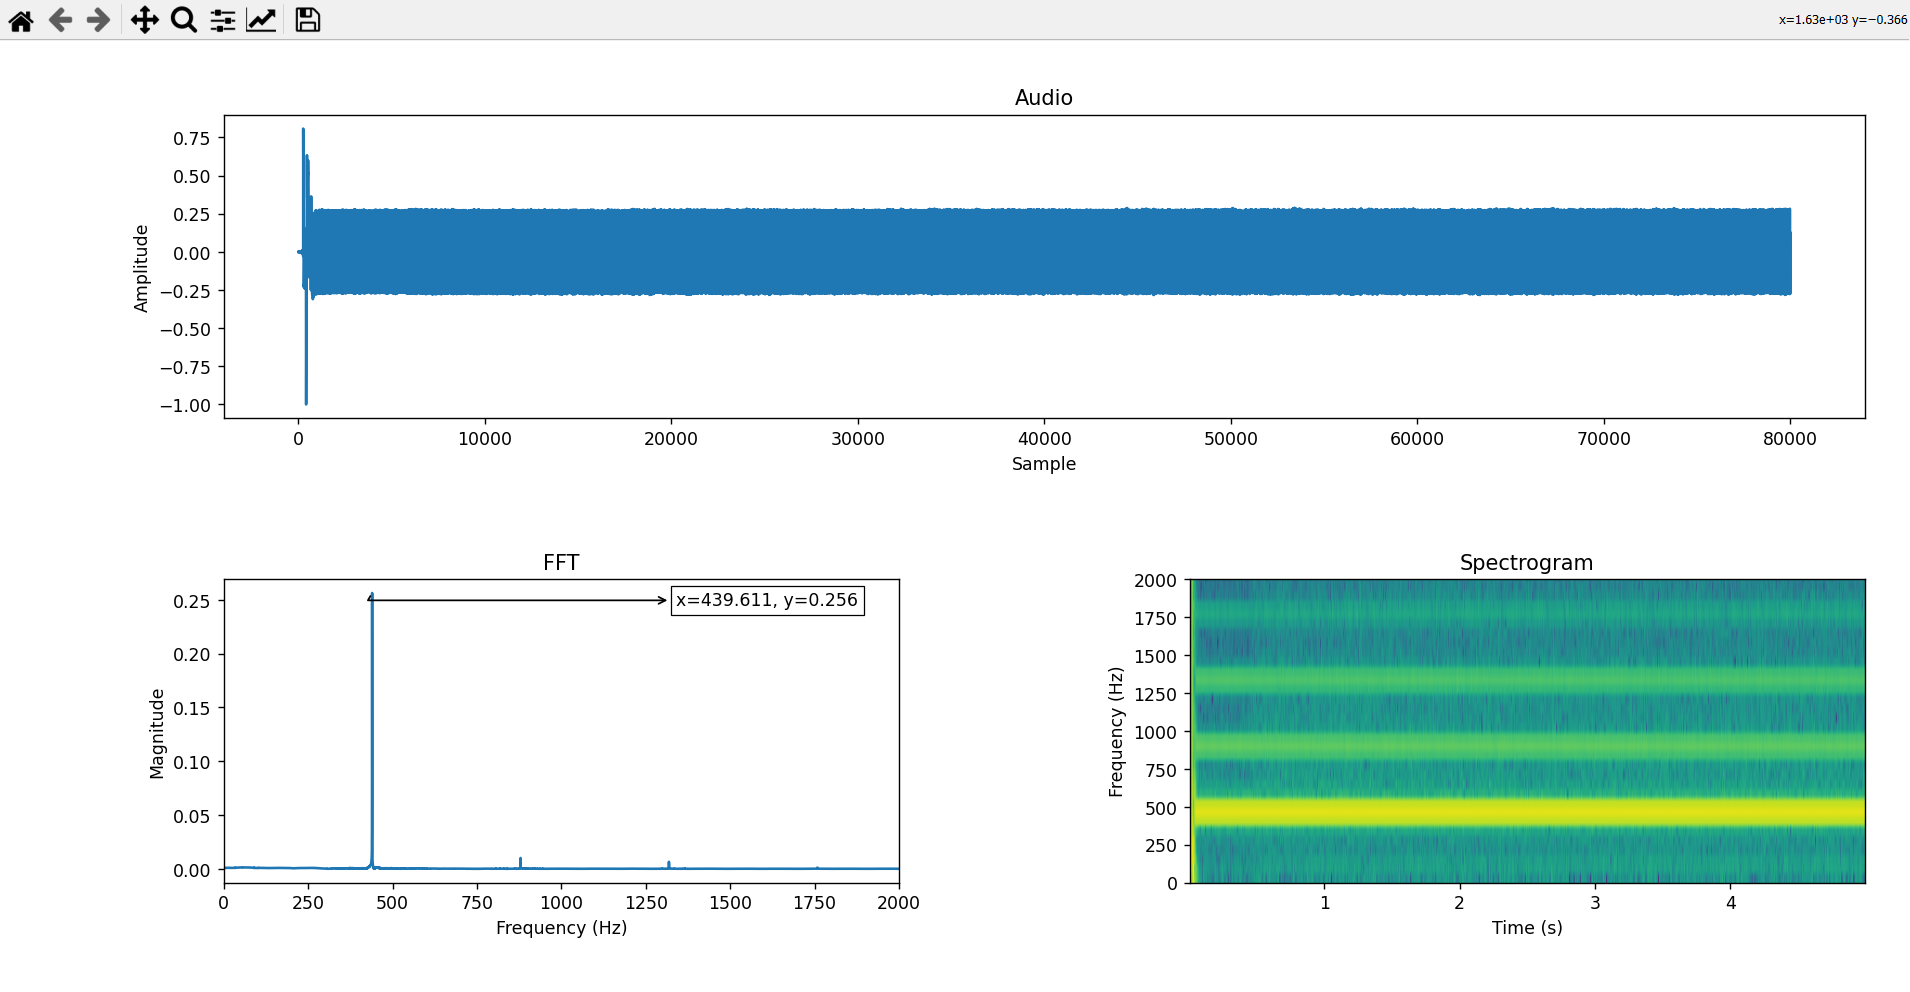
\includegraphics[width=\linewidth]{imgs/analyse_example}
	\caption{Primjer prikaza analize zvučnog zapisa}
	\label{fig:analyse_example}
\end{figure}

\section{Odnos intenziteta zvuka i udaljenosti}

Za analizu ovisnosti intenziteta zvuka o udaljenosti potrebno je pri konstantnoj frekvenciji periodično mijenjati udaljenost i mjeriti intenzitet zvuka u svakoj iteraciji. Za zvuk je odabran ton A4, odnosno zvuk s konstantnom frekvencijom od 440 Hz. Početna udaljenost izvora zvuka od mikrofona je 5 centimetara, a povećavana je za 5 centimetara u svakoj iteraciji sve do udaljenosti od 100 centimetara, odnosno 1 metra. 

Za dobivanje intenziteta svakog zvučnog zapisa korišten je \textit{Audacity}, programski paket otvorenog koda za snimanje i  uređivanje audio signala. Program nudi mogućnost analize frekvencije zvučnog zapisa i iscrtavanja grafa ovisnosti intenziteta zvuka o frekvenciji. Za dobivanje željene vrijednosti intenziteta potrebno je iz iscrtanog grafa u programu pročitati tu vrijednost pri frekvenciji od 440 Hz. Nula je postavljena za maksimalnu glasnoću, stoga su vrijednosti intenziteta zvuka prikazani u negativnoj skali. 

Provedena je analiza nad 20 zvučnih zapisa i dobivene su vrijednosti grafički prikazane u donjoj tablici. 

\begin{tikzpicture}
	\begin{axis}[
		title = {Graf ovisnosti intenziteta zvuka o udaljenosti},
		xlabel=Udaljenost (cm),
		ylabel=Intenzitet zvuka (dB),
		width = \textwidth,
		height = 0.5\textwidth]
		\addplot table [y=L, x=$d$]{data.dat};
	\end{axis}
\end{tikzpicture}

Analizom grafa može se uočiti da postoji obrnuto proporcionalna ovisnost između intenziteta zvuka i udaljenosti izvora od mikrofona - što je izvor dalji od mikrofona, to je intenzitet slabiji. Dobiveni rezultati u skladu su sa zakonom inverznog kvadrata, koji tvrdi da je određena fizikalna veličina obrnuto proporcionalna kvadratu udaljenosti od izvora te fizikalne veličine: 

\begin{equation}
	intenzitet \propto \dfrac{1}{{udaljenost}^2}
\end{equation}



\section{Obrada zvučnih zapisa hrkanja}

Hrkanje je čest poremećaj koji pogađa 20-40\% opće populacije. Ono nastaje kao posljedica vibracije anatomskih struktura u dišnom putu. Treperenje mekog nepca odgovorno je za grubi aspekt zvuka hrkanja. Na hrkanje utječu mnogi faktori kao što su položaj tijela, faza spavanja, dišni putevi i prisutnost ili odsutnost poremećaja disanja tijekom spavanja. Pojava hrkanja može varirati tijekom noći \cite{pevernagie}. 

Iako se hrkanje općenito doživljava kao društvena smetnja, ocjena njegove bučnosti subjektivna je i stoga nedosljedna. Objektivna procjena hrkanja važna je za procjenu učinka terapijskih intervencija. Štoviše, hrkanje nosi informacije koje se odnose na mjesto i stupanj opstrukcije gornjih dišnih putova.

\subsection{Anatomija hrkanja}
Gornji dišni putovi su područje od nosnica i usana do glasnica. Sastoje se od nosne i usne šupljine, ždrijela i gornjeg dijela grkljana. Ždrijelo je stražnji dio glave i sadrži nekoliko anatomskih orijentira, kao što su meko nepce (velum), nepčani krajnici, korijen jezika i nepčana resica (epiglotis). Epiglotis odvaja ždrijelo od jednjaka i grkljana, koji sadrži glasnice \cite{snoringml}.

\begin{figure}[ht]
	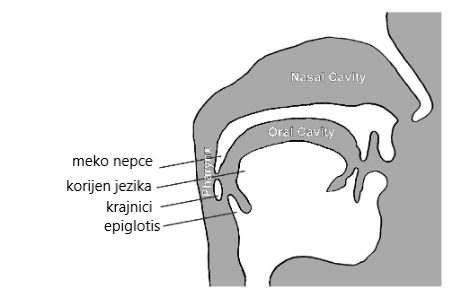
\includegraphics[width=\linewidth]{imgs/anatomy}
	\caption{Anatomija gornjih dišnih puteva \cite{snoringml}}
	\label{fig:anatomy}
\end{figure}

Hrkanje je uzrokovano vibracijama struktura mekog tkiva u gornjim dišnim putovima, osobito na fiziološkim suženjima. 
Tijekom sna, tonus mišića se smanjuje, a meko tkivo opušta, povećavajući njegovu sklonost vibriranju. Brzina protoka zraka pri udisaju povećava se u uskim dijelovima gornjih dišnih puteva, izazivajući vibracije tkiva i strujanja zraka, što zauzvrat uzrokuje hrkanje.

Tipična područja koja pridonose stvaranju zvuka hrkanja su meko nepce i njegov vrh, uvula, koja može vibrirati u anteriorno-posteriornom smjeru, nepčani krajnici koji obično vibriraju u lateralnom smjeru, korijen jezika koja može pasti natrag i ograničiti prolaz prema stražnjoj stijenci ždrijela i epiglotis, koji se može spustiti zbog smanjene strukturne krutosti ili zbog stražnjeg pomaka prema stražnjoj stijenci ždrijela.

Za ciljano liječenje hrkanja i srodnih poremećaja disanja povezanih sa spavanjem, ključno je identificirati mehanizme i mjesta koja doprinose sužavanju dišnih puteva i uzrokuju hrkanje ili respiratorne opstrukcije kod pojedinog subjekta.

%\subsection{Klasifikacija hrkanja}

Široko korištena definicija raznih mehanizama hrkanja je VOTE klasifikacija, koja razlikuje četiri razine u kojima se mogu pojaviti hrkanje i sužavanje dišnih puteva:
\begin{itemize}
	\item V - \textit{Velum}: razina mekog nepca, 
	\item O - \textit{Oropharynx}: razina usnog dijela ždrijela,  
	\item T - \textit{Tongue}: razina korijena jezika, 
	\item E - \textit{Epiglottis}: razina epiglotisa. 
\end{itemize}

U radu \cite{bib} uspoređeni su zvukovi hrkanja izazvani tijekom nazendoskopije s onima u prirodnom snu pomoću spektra zvučnih frekvencija. Pacijenti s palatinalnim hrkanjem tijekom nazendoskopije u snu imali su srednju vršnu frekvenciju od 137 Hz. Najveća frekvencija hrkanja u korijenu jezika bila je 1243 Hz, a kombinirano hrkanje nepca i jezika 190 Hz. Središnje frekvencije bile su 371, 1094 i 404 Hz. Epiglotično hrkanje imalo je vršnu frekvenciju od 490 Hz. Iako rezultati pokazuju da inducirano hrkanje sadrži komponentu više frekvencije zvuka koja nije vidljiva tijekom prirodnog hrkanja, korelacija je dovoljno dobra za kategoriziranje zvučnih zapisa hrkanja. 

Također, visina zvuka hrkanja u niskofrekventnom rasponu (<500 Hz) odgovara osnovnoj frekvenciji s pripadajućim harmonicima. Visina hrkanja određena je vibracijom mekog nepca, dok je nepalatalno hrkanje više „nalik buci“ i ima raspršeniju energiju u višim spektralnim podpojasevima (>500 Hz).

\subsection{Analiza zvučnih zapisa}

Budući da pri snimanju zvuka mikrofon snimi i neželjene frekvencije, potrebno ih je filtrirati. Za filtriranje odabrana je frekvencija od 50 Hz, što je frekvencija gradske mreže u Hrvatskoj i uzročnik najviše smetnji pri obradi zvučnog signala. Slike \ref{fig:with_notch} i \ref{fig:without_notch} prikazuju bitne razlike u očitanim frekvencijama. Na Slici \ref{fig:without_notch}, koja prikazuje graf bez primjene filtra, vidljivo je da je maksimalna vrijednost na frekvenciji oko 50 Hz, što je upravo frekvencija koja je odabrana za filtriranje. Slika \ref{fig:with_notch} prikazuje graf s primjenom \textit{notch} filtra (pojasna brana), i na njoj se jasno vidi koja je stvarna frekvencija za maksimalnu vrijednost grafa. 

\begin{figure}[ht]
	\begin{minipage}[t]{0.5\textwidth}
		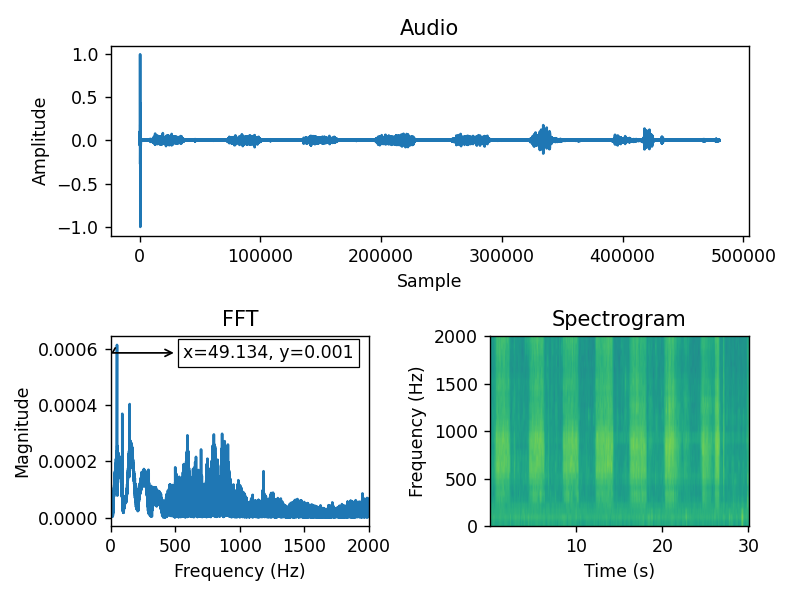
\includegraphics[width=\linewidth]{imgs/without_notch}
		\caption{Analiza bez \textit{notch} filtra}
		\label{fig:without_notch}
	\end{minipage}
	\hspace*{\fill}
	\begin{minipage}[t]{0.5\textwidth}
		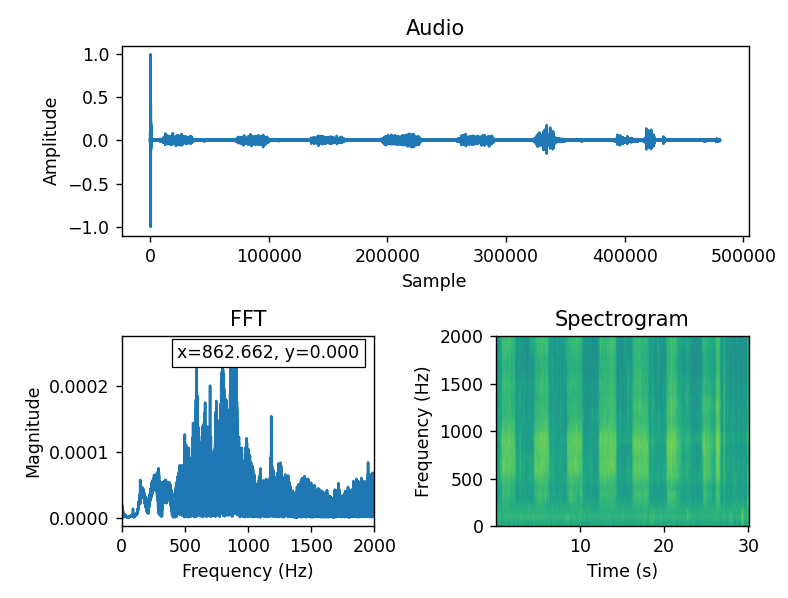
\includegraphics[width=\linewidth]{imgs/with_notch}
		\caption{Analiza s \textit{notch} filtrom}
		\label{fig:with_notch}
	\end{minipage}
\end{figure}

Pojasna brana je pojasni filtar koji kroz većinu frekvencija ostane nepromijenjen, ali prigušuje one u određenom rasponu. Suprotan je propusnom filtru koji ima cilj propuštanja željenih frekvencija. Pojasni filtri odbijaju odnosno prigušuju signale u određenom frekvencijskom pojasu koji se naziva frekvencijski raspon zaustavnog pojasa i propuštaju signale iznad i ispod tog pojasa \cite{notch}.  U nastavku je prikazana prijenosna funkcija filtra:

\begin{equation}
	H(s) = \dfrac{s^2 + \omega_0^2}{s^2 + \omega_c s + \omega_0^2}
\end{equation}

gdje je \(\omega_0\) središnja frekvencija koju se želi ukloniti, a \(\omega_c\) je širina odbijenog frekvencijskog pojasa.  Funkcija \lstinline|iirnoch()| prima središnju frekvenciju za ukloniti, faktor kvalitete i frekvenciju uzorkovanja. Funkcija vraća dva koeficijenta koje prima funkcija \lstinline|filtfilt()|. Ova funkcija primjenjuje linearni digitalni filtar na ulazni signal. Dobivenim koeficijentima koji služe kao brojnik i nazivnik prijenosne funkcije filtrira ulazni signal i vraća ga u filtriranom obliku nad kojim se dalje može pozvati funkcija za Fourierovu transformaciju \cite{scipy}. 

\begin{lstlisting}[language=Python, caption={Primjena \textit{notch} filtra i Fourierove transformacije}]
	b, a = iirnotch(50, 50/len(samples), sampling_rate)
	notch = filtfilt(b, a, samples)
	yf = fft(notch)
	xf = np.linspace(start=0.0, stop=1.0/(2.0*T), num=n//2)
\end{lstlisting}

Razvojnim sustavom STM32WB5MM-DK snimljeno je 27 zvučnih zapisa hrkanja različitih osoba. Budući da je vrlo malen uzorak, zvučni zapisi podijelit će se isključivo na palatalno i nepalatalno hrkanje. Od snimljenih zvučnih zapisa samo su 4 imala frekvenciju hrkanja 500 Hz ili niže, što znači da nepalatalno hrkanje unutar odabranog uzorka daleko učestalije od palatalnog.

Uzme li se u obzir istraživanje vezano uz nazoendoskopiju, 4 zvučna zapisa su kombinirano hrkanje nepca i jezika, dok njih 11 pripada kategoriji hrkanja u korijenu jezika. Ostali zapisi nemaju frekvencije koje su usporedive s rezultatima ovog istraživanja.